%
% Chapter 2
%

\chapter{Theoretical motivation}
\label{theory}

The SM is a set of mathematical formulae and measurements describing elementary particles and their interactions. The intrinsic angular momentum (spin) of the elementary particles is used to classify them. Elementary particles with half-integer spin $(\frac{1}{2}, \frac{3}{2}, \frac{5}{2}, \ldots)$, are classified as fermions, while particles with integer spin (0, 1, 2, ...) are classified as bosons. Quarks and leptons constitute matter and are fermions. There are six quark flavors: up (u), down (d), strange (s), charm (c), bottom (b), and top (t). There are three different types of charged leptons: electron (\Pe), muon (\Pgm), and tau (\Pgt). Each lepton has its corresponding neutral partner: electron neutrino ($\nu_{e}$), muon neutrino ($\nu_{\Pgm}$), and tau neutrino ($\nu_{\Pgt}$). The six flavors of leptons and quarks can be arranged into three generations.

Every fermion has a corresponding anti-particle with the same mass and flipped quantum numbers. Elementary particles of the SM can be seen in Figure~\ref{fig:sm_particles}. The electromagnetic, weak, and strong interactions are part of the SM and can be described as quantum fields. Their interactions are mediated by the gauge bosons, which are spin-one particles. Quantum electrodynamics (QED) is the relativistic quantum field theory (QFT) of the electromagnetic force. The electroweak theory is the unified theory of weak interaction and electromagnetism. The theory of strong interaction is called quantum chromodynamics (QCD).

\begin{figure}[htbp]
  \centering
  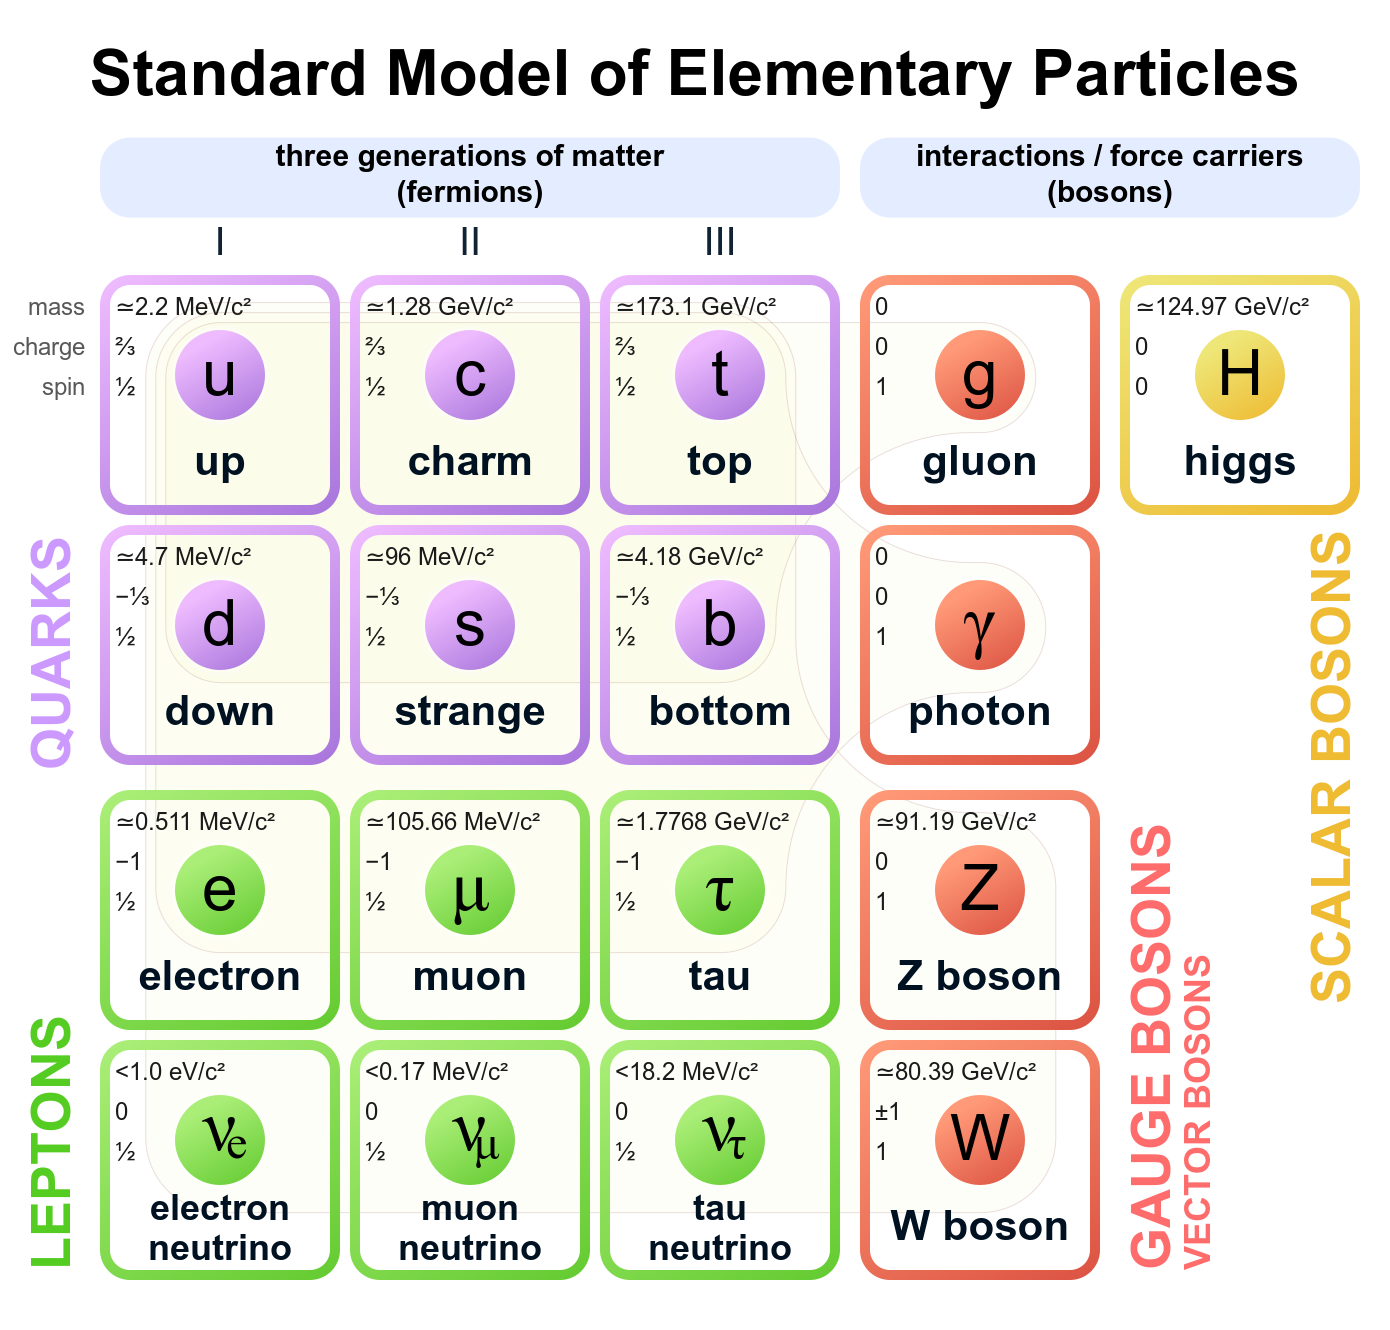
\includegraphics[width=0.8\textwidth]{plots/chapter2/sm_particles.png}
  \caption{Elementary particles of the SM.}
  \label{fig:sm_particles}
\end{figure}


\section{Theoretical building blocks}
The SM is a renormalizable QFT and has a $\suthree \times \sutwo \times \uone$ symmetry structure. The group theory aims to understand the general, abstract details of structures. The Lagrangian describes the dynamics of a system. A type of QFT is a gauge theory, where gauge fields require symmetry under local transformations. In the following paragraphs, a brief overview of groups and Lagrangian is given, and their application in a QFT is described.

A group is a set, G, together with an operation $\star$ that combines any two elements $a$ and $b$ to form another element, denoted $a \star b$. The set and operation, (G, $\star$), must satisfy four requirements to qualify as a group: closure, associativity, the existence of an identity element, and an inverse element. A group is Abelian if the group's elements commute under the group operation $(a \star b = b \star a)$. If the elements do not commute, the group is called non-Abelian. The number of elements in the group determines the order $n$ of the group. A group can be represented in terms of $n \times n$ matrices.

Lie groups are a special type of groups that are parameterized by one or more continuous variables. The transformation of elements in Lie groups can be described as matrices M. These matrices are unitary if the Hermitian conjugate is also the inverse of the transformation, $\text{M}^{\dagger}=(\text{M}^{*})^{\text{T}}=\text{M}^{-1}$. A unitary group is a set of such $n \times n$ matrices that preserve the norm under transformations and correspondingly the probability amplitude. If the unitary matrix's determinant is $\operatorname{det}|\text{M}|=1$, then the volume is preserved under such transformations. A set of such matrices form the special unitary group $\text{SU}(n)$.

The Lagrangian gives the information about the dynamics of a system as a function of generalized coordinates $q$ and their time derivatives $\dot{q}$. In classical physics, the Lagrangian is defined as the kinetic energy minus the potential energy $L=T(q, \dot{q})-V(q)$. In a field theory, the Lagrangian is replaced by the Lagrangian density $\mathcal{L}$, which is a function of the fields $\phi(x^{\Pgm})$, which are functions of spacetime and their derivatives $\partial_{\mu} \phi$. The action $S$ of the system is defined as $S=\int \text{d}^{4} x \mathcal{L}$.

In quantum mechanics, space is treated as an operator, and time is treated as a parameter. In a relativistic theory, space and time have to be treated on an equal footing. QFT interprets the fields as operators parameterized by the spacetime coordinates. It is impossible to measure both the field and its time rate of change simultaneously to infinite precision at a given spacetime point. The vacuum is the state with the lowest possible energy level. When a field operator acts on the vacuum, it produces a state with some energy.

The Lorentz group is the group of all Lorentz transformations of Minkowski spacetime. The Lorentz group contains two copies of the SU(2) group, where the SU(2) group represents spin. The spin of the particle $j$ characterizes the different representations. The Lorentz group can be represented by $(j, j^{\prime})$ for each of the two SU(2) subgroups. There are three important representations of the Lorentz group:

\begin{itemize}
\item The $(0, 0)$ scalar representation.
\item The $(\frac{1}{2}, 0) \oplus(0, \frac{1}{2} )$ left-handed/right-handed spinor representations.
\item The $(\frac{1}{2}, \frac{1}{2} )$ vector representation.
\end{itemize}

Spin is a rotation in the spinor space of SU(2). The spin-0 fields are called scalar fields. Complex scalar fields have the form $\phi = \phi_{1} + i \phi_{2}$, with two real degrees of freedom and hence the fields $\phi$ and $\phi^{\dagger}$ are treated independently.

The spin-1/2 fields are called spinor fields $\Psi$. The left-handed $\Psi_{L}$ and right-handed $\Psi_{R}$ spinors transform the same under rotations but differently under boosts. The adjoint spinor $\bar{\Psi}=\Psi^{\dagger} \gamma^{0}$ has to be defined to have Lorentz invariant terms in the Lagrangian density. The matrices satisfy the anti-commutation relation (Clifford algebra):
%
\[ \left\{\gamma^{\mu}, \gamma^{\nu}\right\}=\gamma^{\mu} \gamma^{\nu}+\gamma^{\nu} \gamma^{\mu}=-2 \eta^{\mu \nu} \mathbb{1} \]
%
with Minkowski metric $\eta^{\mu \nu}$.

A particular type of Lorentz transformations called Parity transformations $\Lambda_{P}$ switches the coordinate frame's handedness. Under parity transformations, left-handed spinors are transformed into right-handed spinors. To be Lorentz invariant, the adjoint field of a left-handed spinor field should be the same as the right-handed spinor field $\bar{\Psi}_{L}=\Psi_{R}$ and vice versa. The field can be projected onto the left and right-handed components using the projection operators: $P_{+} \Psi=\Psi_{R}$ and $P_{-} \Psi=\Psi_{L}$. The charge conjugation is another important transformation: $\Psi \to C \bar{\Psi}^{T}=-i \gamma^2 \Psi^{*}$, which swaps the charge of the field.

The spin-1 fields are called vector fields \amu. Under Lorentz transformations the four components of the vector fields transform as a spacetime vector. The Lorentz invariant terms are:

\begin{equation}
  \amu \text{A}^{\mu}, \quad (\partial_{\mu} \text{A}_{\nu})(\partial^{\mu} \text{A}^{\nu}), \quad (\partial_{\mu} \text{A}^{\mu})(\partial_{\nu} \text{A}^{\nu})
\end{equation}

In QFT, the fundamental fermions are represented as spinor fields, while the gauge bosons are represented as vector fields. An interaction term in the combined Lagrangian densities of both fields leads the two fields to interact. Such a term can be introduced using gauge theory.

Gauge theories are theories in which the Lagrangian is invariant under a continuous group of local transformations with a spacetime dependence. The possible transformations are associated with a Lie group. The elements of a group can be expressed in terms of the group generators. The Lagrangian density of a fermion field is defined to satisfy the Dirac equation. To make the Lagrangian density invariant under a local gauge transformation, a new vector field \amu has to be introduced for each group generator. The vector field can be expressed in terms of the group generators, $\amu=\amu^{a} \ta$, and the gauge bosons are the quanta of these fields.

The derivative $\partial_{\mu}$ in the Lagrangian density is replaced by the covariant derivative $D_{\mu}$, which is $\partial_{\mu}$ along with a term proportional to a gauge field. The second term of the covariant derivative introduces the interaction terms. The vector field dynamics can be included with a kinetic term proportional to the fields' derivatives. The local gauge symmetry is broken if the Lagrangian has terms proportional to $\amu \text{A}^{\mu}$, hence the vector fields are required to be massless. The general principle of local gauge invariance can be used to derive all fundamental interactions of the SM. In the SM, the \PW and \PZ bosons acquire their mass through the Higgs mechanism, which combines the principles of gauge theory and spontaneous symmetry breaking.

When a local symmetry is broken, the gauge fields can acquire mass. A global symmetry that is broken results in massless bosons called Goldstone bosons~\cite{Goldstone:1961eq, Goldstone:1962es}. If we consider a complex scalar field with a Lagrangian that has a local \uone symmetry and a potential with the vacuum $V_{\text{minimum}}$, then choosing a particular ground state breaks the system's symmetry and is considered ``spontaneous'' because there are no external means by which this occurs. After a change of basis, the field is expanded around the constant vacuum value, writing the fields in terms of fluctuations around the chosen vacuum. We can choose the vacuum for a local U(1) symmetry so that the vacuum is real and that $\phi$ is always real; therefore, $\phi$ can be expanded as $\phi = v + \text{H}$, with H being a real scalar field. When a local \uone symmetry is broken, it results in a real scalar with a mass, and the field \amu, originating from the local gauge symmetry, acquires mass.


\section{The Standard Model}
The SM is a non-Abelian gauge theory based on the group $\col \times \iso \times \hyp$, where C stands for color, L indicates that the interaction only involves left-handed states, and Y stands for the hypercharge. The transformations in the color space are represented by the group \col and described by QCD. QCD describes the strong interaction mediated by eight gauge bosons ($\gmu^{a}$) called gluons. Quarks are described as a triplet of spinors that differ in color (red, blue, or green).

\begin{equation}
  \begin{array}{|l|l|c|c|}
    \hline \text { Group } & \text { Operation } & \text { Coupling } & \text { Vector field } \\
    \hline \hyp & \text { Phase } & g^{\prime} & \bmu \\
    \hline \iso & \text { Weak isospin } & g & \wmu^{a} \\
    \hline \col & \text { Color } & g_{S} & \gmu^{a} \\
    \hline
  \end{array}
  \label{tab:group}
\end{equation}

The electroweak theory is represented by the group $\iso \times \hyp$. The neutrinos only interact via the weak interaction, which is represented by \iso. As only left-handed fields interact under \iso, only a left-handed neutrino is needed. The left-handed and right-handed fields can interact under the \hyp group, therefore charged leptons have to exist in both a left-handed and a right-handed state. Left-handed doublet fields
%
\begin{equation}
  \psi_{L}=\left(\begin{array}{l}
  \nu_{e} \\
  e_{L}
  \end{array}\right)
\end{equation}
%
and right-handed singlet fields $e_{R}$ are introduced. The group \iso has three associated gauge fields $\wmu^{a}$ and the group \hyp has one gauge field \bmu. The symmetry groups, couplings, and the associated vector fields are summarized in Table~\ref{tab:group}.

The Higgs field is a complex scalar $\iso \times \hyp$ doublet field. The Higgs boson is a spin-0 particle and is the field quanta of the Higgs field. The Higgs boson's fundamental vertices with the fermions, the gauge bosons of the weak interaction, and its self-interactions can be seen in Figure~\ref{fig:h_vertices}. The Higgs mechanism breaks the electroweak theory into two separate forces: the broken weak theory and the unbroken theory of electromagnetism associated with the $\uone_{em}$ symmetry of QED. The resulting fields $\amu, \wmu^{\pm}$, and $\zmu^{0}$ are linear combinations of the vector fields of $\iso \times \hyp$:
%
\begin{equation}
  \begin{aligned}
    \amu&=\sin \theta_{W} \wmu^{3}+\cos \theta_{W} \bmu \\
    \wmu^{\pm}&=(\wmu^{1} \mp i \wmu^2) / \sqrt{2} \\
    \zmu^{0}&=-\cos \theta_{W} \wmu^{3}+\sin \theta_{W} \bmu
  \end{aligned}
\end{equation}
%
with the weak mixing angle $\theta_{W}=\tan ^{-1}(\frac{g^{\prime}}{g})$, $\sin \theta_{W}=g^{\prime} / \sqrt{g^2+g^{\prime 2}}$ and $\cos \theta_{W}=g / \sqrt{g^2+g^{\prime 2}}$ written in terms of the couplings $g$ of \iso and  $g^{\prime}$ of \hyp. The weak mixing angle relates the strength of the weak and electromagnetic interaction. Furthermore, the electromagnetic coupling $e$ of $\uone_{em}$ is given by $e \equiv g \sin \theta_{W}$.

\begin{figure}[htbp]
  \centering
  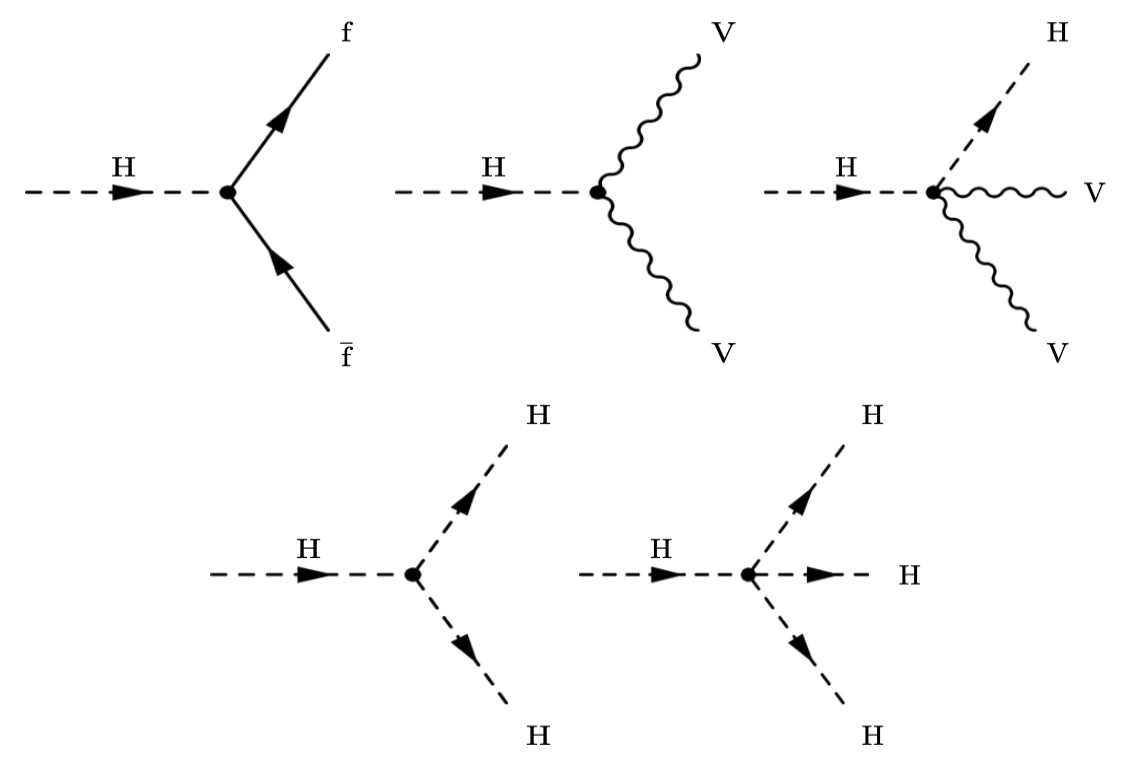
\includegraphics[width=0.8\textwidth]{plots/chapter2/h_vertices.png}
  \caption{Fundamental vertices of the Higgs boson. Fermions are denoted $\text{f}$, anti-fermions are denoted $\bar{\text{f}}$, and gauge bosons of the weak interaction are denoted $\text{V}$.}
  \label{fig:h_vertices}
\end{figure}

\subsection{Electroweak symmetry breaking and the Higgs boson}
For the Higgs mechanism, an arbitrary scalar potential
%
\begin{equation}
  V(\Phi)=\mu^2 \Phi^{\dagger} \Phi+\lambda(\Phi^{\dagger} \Phi)^2
\end{equation}
%
with a self-interacting scalar doublet field $\Phi$ is introduced. The term with the coefficient $\mu^2$ is the mass term of the field. The scalar doublet field $\Phi$ has four degrees of freedom, which are the CP-even and CP-odd components $\phi^{0}$ and $a^{0}$, and the complex charged component $\phi^{+}$:

\begin{equation}
  \Phi=\frac{1}{\sqrt{2}}\left(
  \begin{array}{c}
    \sqrt{2} \phi^{+} \\
    \phi^{0}+i a^{0}
  \end{array}\right)
\end{equation}

For $\mu^2<0$, the scalar doublet field's neutral component acquires a non-zero vacuum expectation value (VEV). Then $\phi^{0}$ can be expanded as $\phi^{0} = v + \text{H}$ with:

\begin{equation}
  \Phi=\frac{1}{\sqrt{2}}\left(
  \begin{array}{c}
    0 \\
    v + \text{H}
  \end{array}\right)
\end{equation}

After electroweak symmetry breaking, the $\col \times \iso \times \hyp$ is broken into a $\col \times \uone_{\text{em}}$. There are three massless Goldstone bosons, which can be identified with three degrees of freedom of the Higgs field. The covariant derivative in the kinematic term couples the Higgs field to the $\wmu^{a}$ and \bmu fields. Thus, the Goldstone bosons mix with the gauge bosons of the corresponding generators of broken symmetries, and the physical \PW and \PZ gauge bosons acquire masses:

\begin{equation}
  \text{M}_{\text{W}}^2=\frac{g^2 v^2}{4}, \quad \text{M}_{\text{Z}}^2=\frac{(g^{\prime 2}+g^2) v^2}{4}
\end{equation}

After electroweak symmetry breaking, there is one remaining degree of freedom of the Higgs field, which is the Higgs boson. The mass of this new scalar particle is given by $\mh = \sqrt{2 \lambda} v$, where $\lambda$ is the self-coupling parameter. One crucial aspect of the electroweak symmetry breaking is the sign of $\mu^2=-\lambda v^2$. The expectation value of the Higgs field is fixed by the Fermi coupling \gf: $v=(\sqrt{2} \gf)^{-1 / 2} \approx 246~\GeV$ which is measured very precisely in muon decays. In the SM, the fermions acquire mass through the Yukawa interactions between the Higgs field and the fermions. The charge conjugated Higgs doublet $\tilde{\Phi}$ is needed to allow interactions with up-type quarks. The Lagrangian of the Yukawa term is given by:
%
\begin{equation}
  \mathcal{L}_{\text {Yukawa }}=-\hat{\lambda}_{d_{i j}} \bar{q}_{L_{i}} \Phi d_{R_{j}}-\hat{\lambda}_{u_{i j} \bar{q}_{L_{i}}} \tilde{\Phi} d_{R_{j}}-\hat{\lambda}_{\ell_{i j}} \bar{\ell}_{L_{i}} \Phi e_{R_{j}}+\text {h.c.}
\end{equation}
%
where $\hat{\lambda}$ are $3 \times 3$ coupling coefficient matrices for the up and down-type quarks and the charged leptons. After electroweak symmetry breaking, the Higgs field acquires a VEV and the fermion mass eigenstate basis is chosen, so that the Higgs interactions are diagonalised: $\hat{\lambda}_{f_{i j}} \to \lambda_{f_{i}} \delta_{i j}$. The mass of the fermions is given by $\text{m}_{f_{i}} = \lambda_{f_{i}} v / \sqrt{2}$, with the corresponding Yukawa coupling $\lambda_{f}$. The Higgs boson was discovered by the ATLAS and CMS collaborations in 2012~\cite{Chatrchyan:2013lba}. Its mass and full width were measured to be $\mh = 125.09 \pm 0.24~\GeV$ and $\Gamma < 1.7~\GeV$.


\section{Lepton flavor violating decays of the Higgs boson}
The SM is considered to be an effective theory up to a certain scale $\Lambda$. The theoretical description of the SM does not incorporate the flavor structure. There are three main puzzles in the SM related to flavor~\cite{Raidal:2008jk}:
\begin{itemize}
  \item The reason for three generations of quarks and leptons.
  \item The principle underlying the formation of the Yukawa matrices describing the SM Yukawa interactions.
  \item The peculiar pattern of fermion masses and mixing.
\end{itemize}

The Yukawa interactions with the Higgs field gives charged leptons their mass. In the SM, LFV decays of the Higgs boson are forbidden because the Yukawa interaction matrix can be diagonalized in the mass basis. The SM extensions like multi-Higgs doublet models can introduce LFV Yukawa couplings along with additional CP-violation. These models can have tree-level Higgs mediated flavor changing neutral currents leading to LFV Yukawa couplings. Also, models like composite Higgs models~\cite{Blankenburg:2012ex} and models with extra dimensions can introduce LFV Yukawa couplings.

A direct mass term of the charged leptons is not gauge invariant, but interactions of the charged leptons to the scalar Higgs field can be introduced with the following term in the Lagrangian:
%
\begin{equation}
  \mathcal{L}_{\text{SM}}=-\lambda_{i j} \overline{L_{L}}^{i} \Phi \ell_{R}^{j}+ \text{h.c.}
\end{equation}
%
where with $\bar{L}_{L}^{i}=(\bar{\nu}_{\ell}^{i}, \bar{\ell}_{L}^{i})$, are the \iso doublets, and $\ell_{R}^{i}$ are the weak singlets with the indices $i, j$ running over generations. After electroweak symmetry breaking, the Higgs doublet can be written in terms of the VEV and the physical Higgs boson leading to the following Lagrangian:
%
\begin{equation}
  \begin{aligned}
    \mathcal{L}_{\text{SM}} &=-\frac{\lambda_{i j}}{\sqrt{2}}(v + \text{H}) \overline{\ell_{L}}^{i} \ell_{R}^{j}+ \text{h.c.} \\
    &=-\frac{\lambda_{i j}}{\sqrt{2}} v \overline{\ell_{L}}^{i} \ell_{R}^{j} - \frac{\lambda_{i j}}{\sqrt{2}} \overline{\ell_{L}}^{i} \ell_{R}^{j} \text{H} + \text{h.c.}
  \end{aligned}
\end{equation}
%
where the term proportional to $\bar{\ell}_{L}^{i} \ell_{R}^{j}$ is the mass term of the charged leptons and the term proportional to $\bar{\ell}_{L}^{i} \ell_{R}^{j} \text{H}$ describes the Yukawa interactions. The mass matrix m, with $\text{m}_{ij}=\frac{\lambda_{ij}}{\sqrt{2}} v$, can be diagonalised using the matrices $V_{L}$ and $V_{R}$:
%
\begin{equation}
  \text{m} = \left(\begin{array}{ccc}
  \text{m}_{e} & 0 & 0 \\
  0 & \text{m}_{\Pgm} & 0 \\
  0 & 0 & \text{m}_{\Pgt}
  \end{array}\right)=\frac{1}{\sqrt{2}} V_{L} \lambda V_{R}^{\dagger} v=\frac{\lambda^{\text{m}}}{\sqrt{2}} v
\end{equation}
%
where $\lambda^{\text{m}}=V_{L} \lambda V_{R}^{\dagger}$ is written in terms of the mass basis. The Yukawa interaction matrix can also be written in terms of the mass basis:
%
\begin{equation}
  \text{Y}=V_{L} \frac{\lambda}{\sqrt{2}} V_{R}^{\dagger}=\frac{\lambda^{\text{m}}}{\sqrt{2}}=\frac{\text{m}}{v}=\left(\begin{array}{ccc}
  \Yee & 0 & 0 \\
  0 & \Ymm & 0 \\
  0 & 0 & \Ytt
  \end{array}\right)
\end{equation}
%
which is also diagonal. Thus, there are no LFV Yukawa interactions in the SM.

\textbf{Dimension-6 operators:} Assuming that the Higgs field is the only field that causes electroweak symmetry breaking and that the particle spectrum is only composed of the SM particles up to an energy scale $\Lambda \gg 200~\GeV$, we can integrate out the additional heavy fields, which gives us an effective field theory. The SM Lagrangian, which has dimension four, can be extended with higher-dimension operators. An effective Lagrangian with additional dimension-6 operators $O_{n}^{i j}$ can be written as:
%
\begin{equation}
  \mathcal{L}_{\text{eff}}=\mathcal{L}_{\text{SM}}+\sum_{\text{n}ij} \frac{\alpha_{\text{n}}^{ij}}{\Lambda^2} O_{\text{n}}^{i j}
\end{equation}
%
where $i, j$ denote flavor indices, n runs over the number of independent operators, $\Lambda$ is the scale of new physics, and $\alpha_{\text{n}}^{i j}$ are coefficients~\cite{DiazCruz:1999xe}.

The effects of new physics at the electroweak scale can be described in a model-independent way using this effective Lagrangian. The effective Lagrangian can also contain a dimension-5 operator, which can generate neutrino masses, but it cannot generate LFV interactions for the Higgs boson. However, LFV interactions of the Higgs boson can be generated using the dimension-6 operator $O_{L \phi}^{i j}=(\Phi^{\dagger} \Phi)(\bar{L}_{i} \ell_{R j} \Phi)$ which is a Yukawa-type operator. The dimension-6 operator also contributes to the fermion mass matrices. After including these contributions in the fermion mass matrices, which are then diagonalized and the interaction term of the Lagrangian is written in terms of the mass basis. The Lagrangian has the following additional term after including the Yukawa-type operator:
%
\begin{equation}
  \Delta \mathcal{L}=-\frac{\lambda_{i j}^{\prime}}{\Lambda^2}(\Phi^{\dagger} \Phi)(\bar{L}_{L}^{i} \ell_{R}^{j} \Phi)+h.c.
\end{equation}
%
where $\lambda_{i j}^{\prime}$ is the coefficient $\alpha_{n}^{i j}$ of the dimension-6 operator $O_{L \phi}^{i j}$.

Electroweak symmetry breaking leads to the following Lagrangian terms:
%
\begin{equation}
  \begin{aligned}
    \Delta \mathcal{L} &=-\frac{\lambda_{i j}^{\prime}}{\Lambda^2}(\frac{v+\text{H}}{\sqrt{2}})^2 \bar{\ell}_{L}^{i} \ell_{R}^{j}(\frac{v+\text{H}}{\sqrt{2}}) \\
    &=-\frac{\lambda_{i j}^{\prime}}{\Lambda^2} \frac{1}{(\sqrt{2})^{3}}(v^{3}+3 v^2 \text{H} + 3 v \text{H}^2 + \text{H}^{3}) \bar{\ell}_{L}^{i} \ell_{R}^{j} \\
    &=-\frac{1}{\sqrt{2}} \frac{\lambda_{i j}^{\prime}}{2 \Lambda^2}(v^{3} \overline{\ell_{L}^{i}} \ell_{R}^{j}+3 v^2 \overline{\ell_{L}^{i}} \ell_{R}^{j} \text{H} + 3 v \bar{\ell}_{L}^{i} \ell_{R}^{j} \text{H}^2+\bar{\ell}_{L}^{i} \ell_{R}^{j} \text{H}^{3})
  \end{aligned}
\end{equation}
%
where the term proportional to $\overline{\ell_{L}^{i}} \ell_{R}^{j}$ leads to an additional mass term of the charged leptons and the term proportional to $\overline{\ell_{L}^{i}} \ell_{R}^{j} \text{H}$ adds a further Yukawa-interaction term. Thus, the mass term of the effective Lagrangian is the sum of the SM mass term and the additional contribution:

\begin{equation}
  \begin{aligned}
    \mathcal{L}_{\text {mass }} &=\mathcal{L}_{\text {mass}, \text{SM}}+\Delta \mathcal{L}_{\text {mass }} \\
    &=-(\frac{\lambda_{i j}}{\sqrt{2}} v+\frac{1}{\sqrt{2}} \frac{\lambda_{i j}^{\prime}}{2 \Lambda^2} v^{3}) \bar{\ell}_{L}^{i} \ell_{R}^{j} \\
    &=-\frac{1}{\sqrt{2}}(\lambda_{i j}+\frac{v^2}{2 \Lambda^2} \lambda_{i j}^{\prime}) v \bar{\ell}_{L}^{i} \ell_{R}^{j}
  \end{aligned}
\end{equation}

The term of the effective Lagrangian which describes the Yukawa interactions is given by:

\begin{equation}
  \begin{aligned}
    \mathcal{L}_{\text{Y}} &=\mathcal{L}_{\text{Y}, \text{SM}}+\Delta \mathcal{L}_{\text{Y}} \\
    &=-(\frac{\lambda_{i j}}{\sqrt{2}}+\frac{1}{\sqrt{2}} \frac{\lambda_{i j}^{\prime}}{2 \Lambda^2} 3 v^2) \bar{\ell}_{L}^{i} \ell_{R}^{j} \text{H} \\
    &=-\frac{1}{\sqrt{2}}(\lambda_{i j}+3 \frac{v^2}{2 \Lambda^2} \lambda_{i j}^{\prime}) \bar{\ell}_{L}^{i} \ell_{R}^{j} \text{H}
  \end{aligned}
\end{equation}

The mass matrix of the charged leptons can be diagonalized as for the SM using other matrices $V_{L}, V_{R}$:

\begin{equation}
  \sqrt{2} \text{m} = V_{L}[\lambda+\frac{v^2}{2 \Lambda^2} \lambda^{\prime}] V_{R}^{\dagger} v
\end{equation}

The Yukawa interaction matrix can then be written in terms of the mass basis:
%
\begin{equation}
  \begin{aligned}
    \sqrt{2} \text{Y} &=V_{L}[\lambda+3 \frac{v^2}{2 \Lambda^2} \lambda^{\prime}] V_{R}^{\dagger} \\
    &=\frac{\sqrt{2} \text{m}}{v}+V_{L} 2 \frac{v^2}{2 \Lambda^2} \lambda^{\prime} V_{R}^{\dagger} \\
    &=\frac{\sqrt{2} \text{m}}{v}+\frac{v^2}{\Lambda^2} V_{L} \lambda^{\prime} V_{R}^{\dagger} \\
    &=\frac{\sqrt{2} \text{m}}{v}+\frac{v^2}{\Lambda^2} \hat{\lambda}
  \end{aligned}
\end{equation}
%
where $\text{m}$ is the diagonal mass matrix and $\hat{\lambda}=V_{L} \lambda^{\prime} V_{R}^{\dagger}$. The first term is the Yukawa term of the SM, while the second term can introduce non-diagonal terms as $\hat{\lambda}$ is in principle an arbitrary non-diagonal matrix, leading to Yukawa couplings \Yij with possible LFV Yukawa interactions:

\begin{equation}
  \text{Y}_{i j}=\frac{\text{m}_{i}}{v} \delta_{i j}+\frac{v^2}{\sqrt{2} \Lambda^2} \hat{\lambda}_{i j}
\end{equation}

\textbf{Type-III 2HDM:} The two Higgs doublet model (2HDM) is one of the most studied extensions of the SM. The structure of Yukawa couplings can characterize them. In Type-I, Type-II, and Type-X 2HDM, each fermion type is coupled to only one scalar doublet. Thus there is no flavor violating Yukawa couplings of the neutral scalar boson in this case. In Type-III 2HDM, however, both of the scalar doublets couple to all the fermions. As a result, there is a possibility of flavor violation in the neutral scalars Yukawa couplings~\cite{Primulando:2016eod}.

In the Higgs basis, the VEV resides only in $\Phi_{1}$ and the fields $\Phi_{1}$ and $\Phi_{2}$ can be expanded as
%
\begin{equation}
  \Phi_{1}=\left(\begin{array}{c} \text{G}^{+} \\ \frac{1}{\sqrt{2}}\left(v+\phi_{1}+i \text{G}^{0}\right) \end{array}\right), \quad
  \Phi_{2}=\left(\begin{array}{c} \text{H}^{+} \\ \frac{1}{\sqrt{2}}\left(\phi_{2}+i \text{A}\right) \end{array}\right)
\end{equation}
%
where $v$ is the VEV, $\text{G}^{\pm}$ and $\text{G}^0$ are the would-be Goldstone bosons, $\text{H}^{\pm}$ is the charged Higgs, A is the neutral CP-odd Higgs, $\phi_{1}$ and $\phi_{2}$ are the neutral CP-even Higgs. The fields $\phi_{1}$ and $\phi_{2}$ are not mass eigenstates. They are related to the mass eigenstates H (SM Higgs boson) and $\text{H}^{'}$ (neutral heavy Higgs boson) by

\begin{equation}
  \left(\begin{array}{l} \phi_{1} \\ \phi_{2} \end{array}\right) = \left(\begin{array}{r} \cos \alpha \quad \sin \alpha \\ -\sin \alpha \quad \cos \alpha \end{array}\right)\left(\begin{array}{l} \text{H} \\ \text{H}^{'} \end{array}\right)
\end{equation}

The Yukawa sector in the Type-III 2HDM is given by
%
\begin{equation}
  \mathcal{L}_{\text{Yukawa}}=-\frac{\sqrt{2} \text{m}_{\ell}^{i}}{v} \delta^{i j} \bar{L}_{L}^{i} \ell_{R}^{j} \Phi_{1}-\sqrt{2} \text{Y}_{\ell}^{i j} \bar{L}_{L}^{i} \ell_{R}^{j} \Phi_{2}
\end{equation}
%
where $\text{m}_{\ell}$ are lepton masses, $\text{Y}_{\ell}$ are the Yukawa coupling matrices, and the indices $i, j, k$ run over lepton families. After electroweak symmetry breaking, the Yukawa couplings in the physical basis read

\begin{equation}
  \begin{aligned}
    \mathcal{L}_{\text{Yukawa}} &\supset -y_{\ell, \text{H}}^{i j} \bar{\ell}_{L}^{i} \ell_{R}^{j} \text{H} - y_{\ell, \text{H}^{'}}^{i j} \bar{\ell}_{L}^{i} \ell_{R}^{j} \text{H}^{'} + \text{h.c.} \\
    y_{\ell, \text{H}}^{i j} &=\frac{\text{m}_{\ell}^{i}}{v} \delta^{i j} \cos \alpha - \text{Y}_{\ell}^{i j} \sin \alpha \\
    y_{\ell, \text{H}^{'}}^{i j} &=\frac{\text{m}_{\ell}^{i}}{v} \delta^{i j} \sin \alpha + \text{Y}_{\ell}^{i j} \cos \alpha
  \end{aligned}
\end{equation}

\textbf{LFV Yukawa couplings:} The inclusion of LFV Yukawa interactions were discussed by introducing a dimension-6 operator to the Lagrangian and in theories with more than one Higgs doublet, where the scalar fields can mix. There are several possible additional terms to the Lagrangian due to new physics, which prevent the simultaneous diagonalization of mass matrix and the Yukawa matrix. Thus, the Yukawa term of the Lagrangian for the charged leptons in the mass basis is after the electroweak symmetry breaking in general given by:
%
\begin{equation}
  \mathcal{L}_{\text{Yukawa}} = -\text{m}_{i} \bar{\ell}_{L}^{i} \ell_{R}^{i} - \text{Y}_{i j} \bar{\ell}_{L}^{i} \ell_{R}^{j} \text{H}+\text{h.c.}
\end{equation}
%
where \Yij are the entries of the Yukawa matrix:
%
\begin{equation}
  \text{Y}=\left(\begin{array}{ccc}
  \Yee & \Yem & \Yet \\
  \Yme & \Ymm & \Ymt \\
  \Yte & \Ytm & \Ytt
  \end{array}\right)
\end{equation}
%
which can have LFV Yukawa couplings \Yij. LFV Yukawa couplings allow LFV decays of the Higgs boson.

The Higgs boson couples to all particles according to their mass in the SM. The LFV Yukawa couplings might be related closely to the fermion mass matrices in the presence of new physics, reflecting the observed fermion mass hierarchy~\cite{Cheng:1987rs}. The LFV couplings then have a hierarchical structure given by $\Delta_{ij} \sqrt{\text{m}_{i} \text{m}_{j}}$, where $i, j$ are the generation indices, and $\Delta_{ij}$ is related to the mass mixing. The mass corrections to the lepton masses coming from mass mixing are assumed to be small in the natural assumption. The SM Yukawa couplings are taken for the flavor diagonal couplings. The LFV branching fractions can be expressed in terms of the SM ones:
%
\begin{equation}
  \BHij = \BHsm \cdot \frac{\text{m}_{\ell_{j}}}{\text{m}_{\ell_{i}}}
\end{equation}
%
with the total decay width asummed to be the SM one, \BHij being the natural branching fraction and \BHsm being the branching fraction for the SM Higgs boson decay to two leptons. The LFV branching fractions are expected to be of similar size or smaller than \BHij. A naturalness assumption referred to as theoretical naturalness limit can also be derived for the Yukawa couplings:

\begin{equation}
  |\Yji \Yij| \lesssim \frac{\text{m}_{i} \text{m}_{j}}{v^2}
\end{equation}


\section{Constraints from low-energy measurements}

Constraints on the Higgs boson's LFV decays have been derived using low-energy measurements and with certain assumptions on the value of flavor diagonal Yukawa couplings. The constraints from several low-energy measurements on LFV Yukawa couplings are discussed in this section. These measurements and the assumptions used to derive constraints on the LFV Yukawa couplings are presented.

\textbf{Constraints from LFV decays \liljg:} LFV Yukawa couplings also contribute to LFV decays of the type \liljg, where $i, j$ are flavor indices with $i \neq j$. One-loop and two-loop diagrams of this process are shown in Figure~\ref{fig:tmg}. Constraints of the type $\sqrt{|\Yij|^2+|\Yji|^2}$ can be derived assuming SM values for \Ytt, \Ymm, and $\text{Y}_{\text{tt}}$. A further constraint on $(|\Ytm \Yet|^2 + |\Ymt \Yte|^2)^{1/4}$ can be obtained from $\Pgm \to \Pe \Pgg$ by setting \Yme and \Yem to zero.

\begin{figure}[htbp]
  \centering
  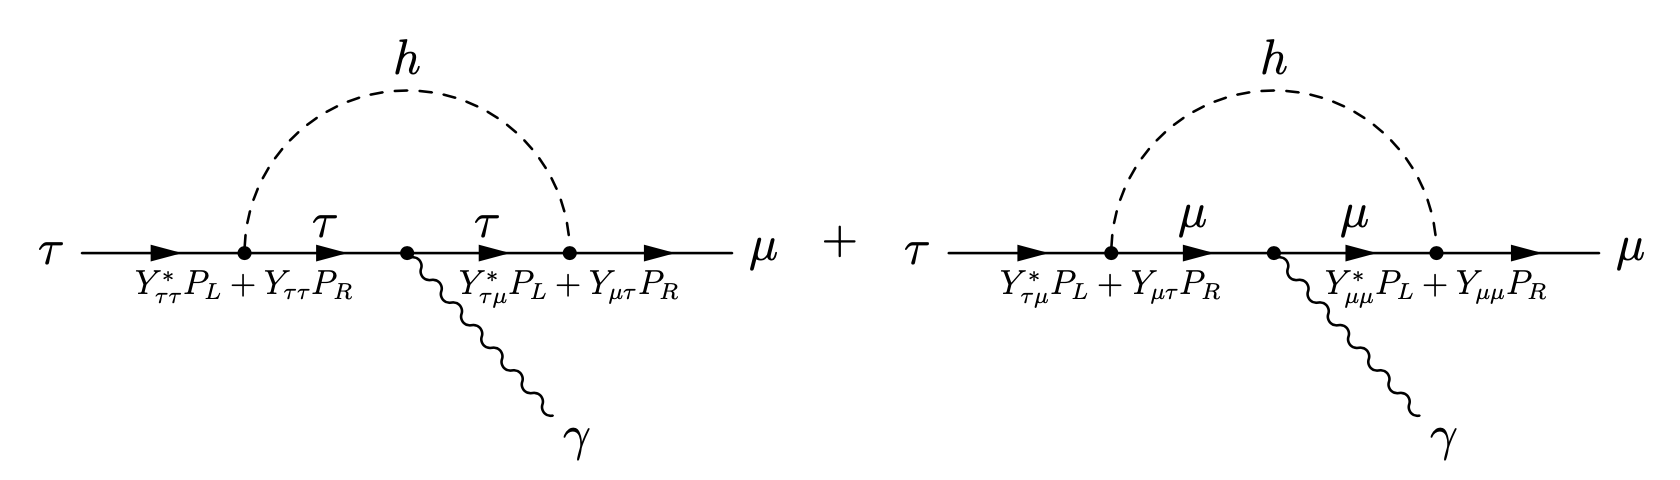
\includegraphics[width=0.8\textwidth]{plots/chapter2/1loop.png} \\
  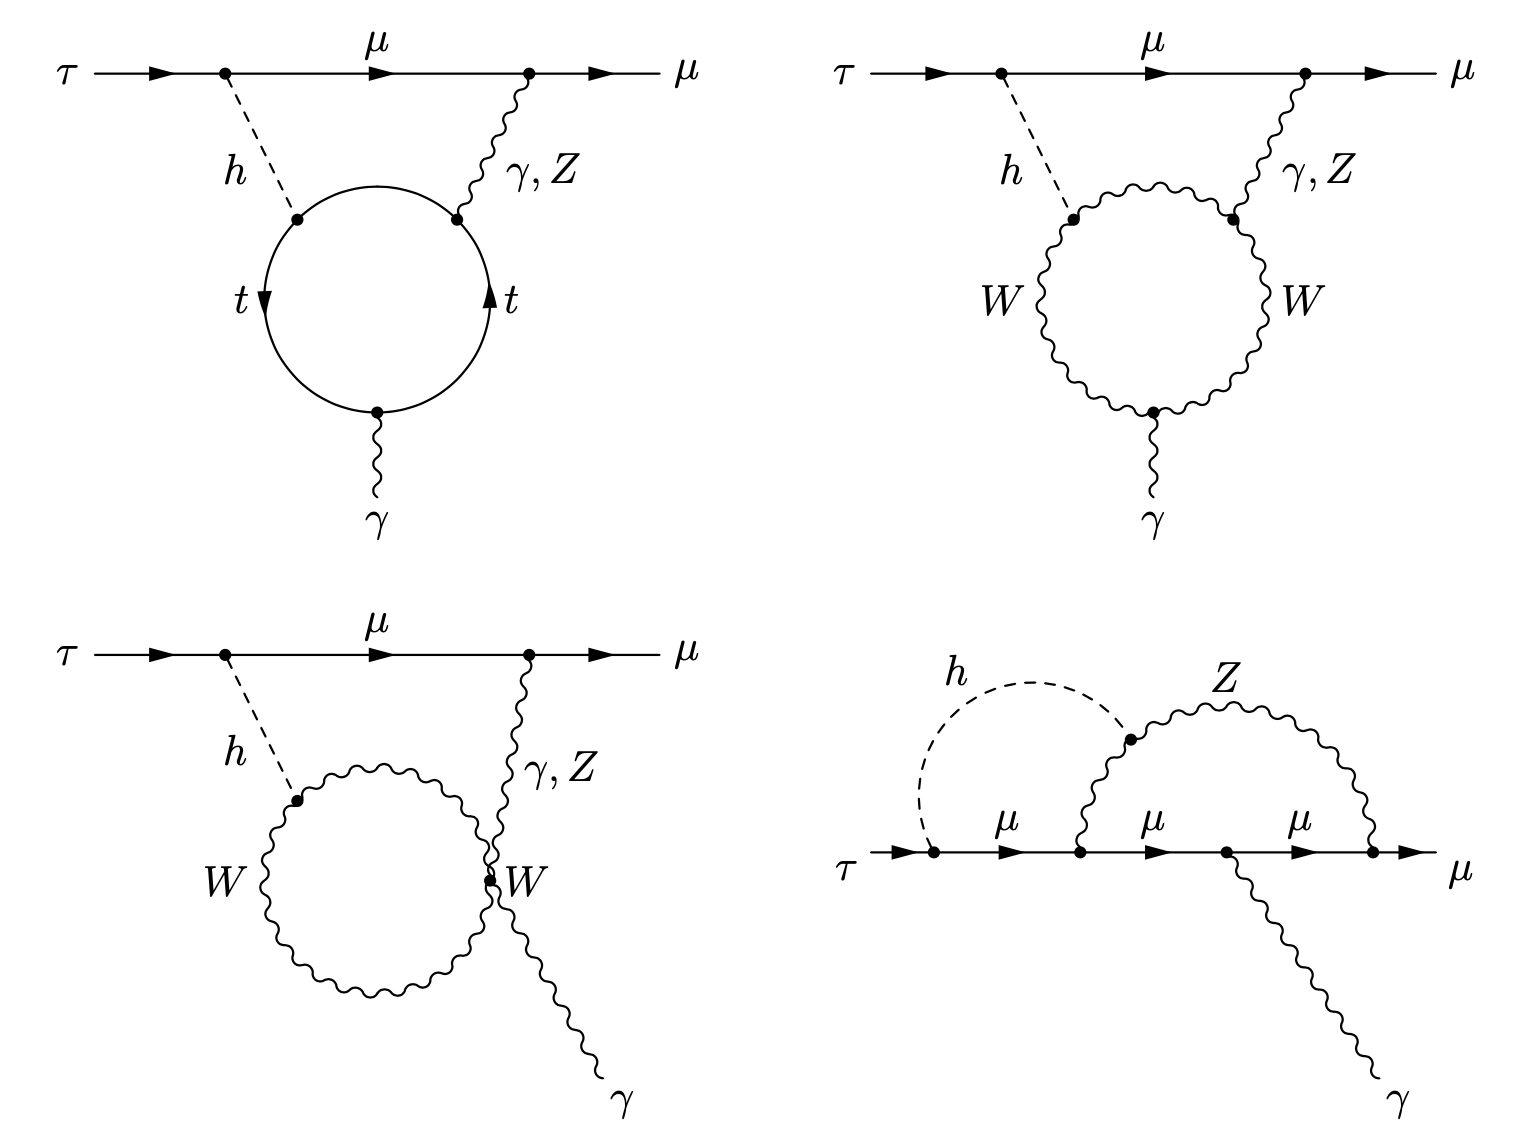
\includegraphics[width=0.8\textwidth]{plots/chapter2/2loop.png}
  \caption{Diagrams contributing to the flavor violating decay $\Pgt \to \Pgm \Pgg$, mediated by a Higgs boson with flavor violating Yukawa couplings.}
  \label{fig:tmg}
\end{figure}

\textbf{Constraints from LFV decays \ltl:} LFV Yukawa couplings also contribute to LFV decays of the type \ltl. Such decays have been searched for and constraints of the type $\sqrt{|\Yij|^2+|\Yji|^2}$ can be derived assuming SM values for \Ytt, \Ymm, and $\text{Y}_{\text{tt}}$. The \PZ boson contribution to the LFV decay $\Pgt \to \Pgm$ are neglected because their contributions are negligible~\cite{Goto:2015iha}.

\textbf{Constraints from muonium-antimuonium oscillations:} The muonium ($M$) bound state $\Pgm^{+} \Pe^{-}$ can oscillate to the antimuonium ($\bar{M}$) bound state $\Pe^{+} \Pgm^{-}$. An upper limit on the conversion probability $P(M \to \bar{M}) < 8.3 \times 10^{-11}$~\cite{Willmann:1998gd} was derived by the muonium-antimuonium conversion spectrometer experiment. The time-integrated conversion probability depends on the mass splitting between the two mass eigenstates of the mixed $M-\bar{M}$ system, which depends on $|\text{Y}_{\Pgm e}+\text{Y}_{e \Pgm}^{*}|$~\cite{Harnik:2012pb}.

\textbf{Constraints from magnetic and electric dipole moments:} The muon's experimental value $g_{\Pgm}-2$ is more than three standard deviations above the SM prediction. Neglecting terms suppressed by $\text{m}_{\Pgm} / \text{m}_{\Pgt}$ or $\text{m}_{\Pgt} / \text{m}_\text{H}$, the LFV contribution to $g_{\Pgm}-2$ due to the one-loop diagram has the form
%
\begin{equation}
  a_{\Pgm} \equiv \frac{g_{\Pgm}-2}{2} \propto \operatorname{Re}(\Ymt \Ytm)
\end{equation}
%
with the discrepancy between measurement and SM prediction having the size
%
\begin{equation}
  \Delta a_{\Pgm} \equiv a_{\Pgm}^{\text{exp}}-a_{\Pgm}^{\text{SM}}=(2.87 \pm 0.63 \pm 0.49) \times 10^{-9}
\end{equation}
%
where $a_{\Pgm}^{\text{exp}}$ and $a_{\Pgm}^{\text{SM}}$ are the measured and predicted value, respectively. The one-loop diagram can contribute to the muon's electric dipole moment if the LFV Yukawa couplings are complex. If the terms suppressed by $\text{m}_{\Pgm} / \text{m}_{\Pgt}$ or $\text{m}_{\Pgt} / \text{m}_\text{H}$ are neglected, the dependence on the LFV Yukawa couplings of the electric dipole moment $d_{\Pgm}$ is

\begin{equation}
  d_{\Pgm} \propto-\operatorname{Im}(\Ymt \Ytm)
\end{equation}

\textbf{Constraints from \mte conversion in nuclei:} LFV Yukawa couplings can also contribute to \mte conversion in nuclei via a tree-level exchange of the Higgs boson and one-loop diagrams with the Higgs boson and a photon exchange. The two-loop diagrams' contribution is larger than the one-loop diagrams because they are only suppressed by the weak gauge coupling or $\mathrm{Y_{tt}}$ and were taken into account for deriving the constraints on the LFV Yukawa couplings.

Constraints on the LFV Yukawa couplings from low-energy measurements are summarized in Table~\ref{tab:indirect}. The LFV decays of type \liljg give the strongest constraints. These measurements constrain the branching fractions of LFV Higgs boson decays to \mutau or \etau to be $\lesssim \mathcal{O}(10^{-1})$, while the constraint for the decay to \emm is stronger and calculated to be $\lesssim \mathcal{O}(10^{-8})$. Constraints on the branching fractions were derived under the assumption that only one of them contributes in addition to the SM Higgs boson's total width.

%%% Low energy constraints
\begin{table}[!hbpt]
\centering
\caption{Constraints on LFV Yukawa couplings from low-energy measurements ~\cite{Harnik:2012pb}.}
\begin{tabular}{ccc}
\hline
\hline
Channel                   & Coupling                   & Bound                 \\
\hline
$\Pgm \to \Pe \Pgg$       & $\sqrt{|\Yme|^2+|\Yem|^2}$ & $<3.6 \times 10^{-6}$ \\
$\Pgm \to 3 \Pe$          & $\sqrt{|\Yme|^2+|\Yem|^2}$ & $\lesssim 3.1 \times 10^{-5}$ \\
electron $g-2$            & Re(\Yem \Yme)              & $-0.019 \ldots 0.026$ \\
electron EDM              & $|Im(\Yem \Yme)|$          & $<9.8 \times 10^{-8}$ \\
$\Pgm \to$ \Pe conversion & $\sqrt{|\Yme|^2+|\Yem|^2}$ & $<1.2 \times 10^{-5}$ \\
$M-\bar{M}$ oscillations  & $|\Yme+\Yem^{*}|$          & $<0.079$ \\
\hline
$\Pgt \to \Pe \Pgg$       & $\sqrt{|\Yte|^2+|\Yet|^2}$ & $<0.014$ \\
$\Pgt \to 3 \Pe$          & $\sqrt{|\Yte|^2+|\Yet|^2}$ & $\leq 0.12$ \\
electron $g-2$            & Re(\Yet \Yte)              & $-2.1 \ldots 2.9 \times 10^{-3}$ \\
electron EDM              & $|Im(\Yet \Yte)|$          & $<1.1 \times 10^{-8}$ \\
\hline
$\Pgt \to \Pgm \Pgg$      & $\sqrt{|\Ytm|^2+|\Ymt|^2}$ & $<0.016$ \\
$\Pgt \to 3 \Pgm$         & $\sqrt{|\Ytm|^2+|\Ymt|^2}$ & $\lesssim 0.25$ \\
muon $g-2$                & Re(\Ymt \Ytm)              & $(2.7 \pm 0.75) \times 10^{-3}$ \\
muon EDM                  & $|Im(\Ymt \Ytm)|$          & $-0.8 \ldots 1.0$ \\
\hline
$\Pgm \to \Pe \Pgg$       & $(|\Ytm \Yet|^2+|\Ymt \Yte|^2)^{1/4}$ & $<3.4 \times 10^{-4}$ \\
\hline
\hline
\end{tabular}
\label{tab:indirect}
\end{table}



\section{Lepton flavor violating decays of the Higgs boson at the LHC}

In the SM, the Higgs boson couples to all particles according to their mass. The branching fraction for Higgs boson decays to taus is in the order of 6\%, and the branching fraction of the Higgs boson to muons is in the order of 0.02\%. The LFV branching fractions are expected to be of the same size or smaller than \BHij using the natural assumption. Furthermore, LFV branching fractions \BHij can be expressed in terms of SM ones. Then, the LFV Higgs boson decay to \mutau should have a natural branching fraction in the order of 0.5\%, between decays to taus and muons. LFV decays of the Higgs boson to \etau would have a smaller natural branching fraction in the order of $0.001\% = 10^{-5}$.

Low-energy measurements indirectly constrain branching fractions of the LFV Higgs boson decays to \mutau or \etau to be smaller than 10\%, which is larger than their natural branching fractions. These constraints were derived, assuming flavor changing neutral currents to be dominated by Higgs boson contributions; therefore, LFV effects could be canceled by other new physics effects leading to weaker limits. Direct searches for LFV decays of the Higgs boson are independent of assumptions on other new physics models.

The CMS experiment published the first direct search for \Hmt~\cite{Khachatryan:2015kon}, followed by searches for \Het and \Hem decays~\cite{Khachatryan:2016rke}, using \pp collision data corresponding to an integrated luminosity of 19.7~\fb at a center-of-mass energy of 8~\TeV. A small excess of data with respect to the SM background-only hypothesis at $\mh = 125~\GeV$ was observed in the \Hmt channel, with a significance of 2.4 standard deviations, and the best fit for the branching fraction was found to be $\BHmt = (0.84^{+0.39}_{-0.37})\%$. A constraint was set on the observed (expected) branching fraction $\BHmt < 1.51\% (0.75\%)$ at 95\% CL. This search has improved the limit on the branching fraction \BHmt from the indirect limit by one order of magnitude.

No excess of events over the estimated background was observed in the \Het or \Hem channels, and observed (expected) upper limits on the branching fractions $\BHet < 0.69\% (0.75\%)$ and $\BHem < 0.035\% (0.048\%)$ at 95\% CL were set. The ATLAS Collaboration reported searches for \Het and \Hmt using \pp collision data at a center-of-mass energy of 8~\TeV, finding no significant excess of events over the background expectation, and set observed (expected) limits of $\BHmt < 1.43\% (1.01\%)$ and $\BHet < 1.04\% (1.21\%)$ at 95\% CL~\cite{Aad:2016blu, Aad:2015gha}.

The CMS experiment placed an upper limit on the observed (expected) branching fraction $\BHmt < 0.25\% (0.25\%)$ and $\BHet < 0.61\% (0.37\%)$ at 95\% CL using the 2016 dataset corresponding to an integrated luminosity of 35.9~\fb~\cite{Sirunyan:2017xzt}. The ATLAS experiment published the search results using the 2016 dataset corresponding to an integrated luminosity of 36.1~\fb and placed an upper limit of 0.28\% (0.37\%) and 0.47\% (0.34\%) on the \BHmt and \BHet with a 95\% CL, respectively~\cite{Aad:2019ugc}. Figure~\ref{fig:bh} shows the expected and observed 95\% CL upper limits for each category and their combination of the search performed by the CMS experiment. Figure~\ref{fig:yukawa} shows the corresponding Yukawa couplings.

\begin{figure}[htbp]
  \centering
  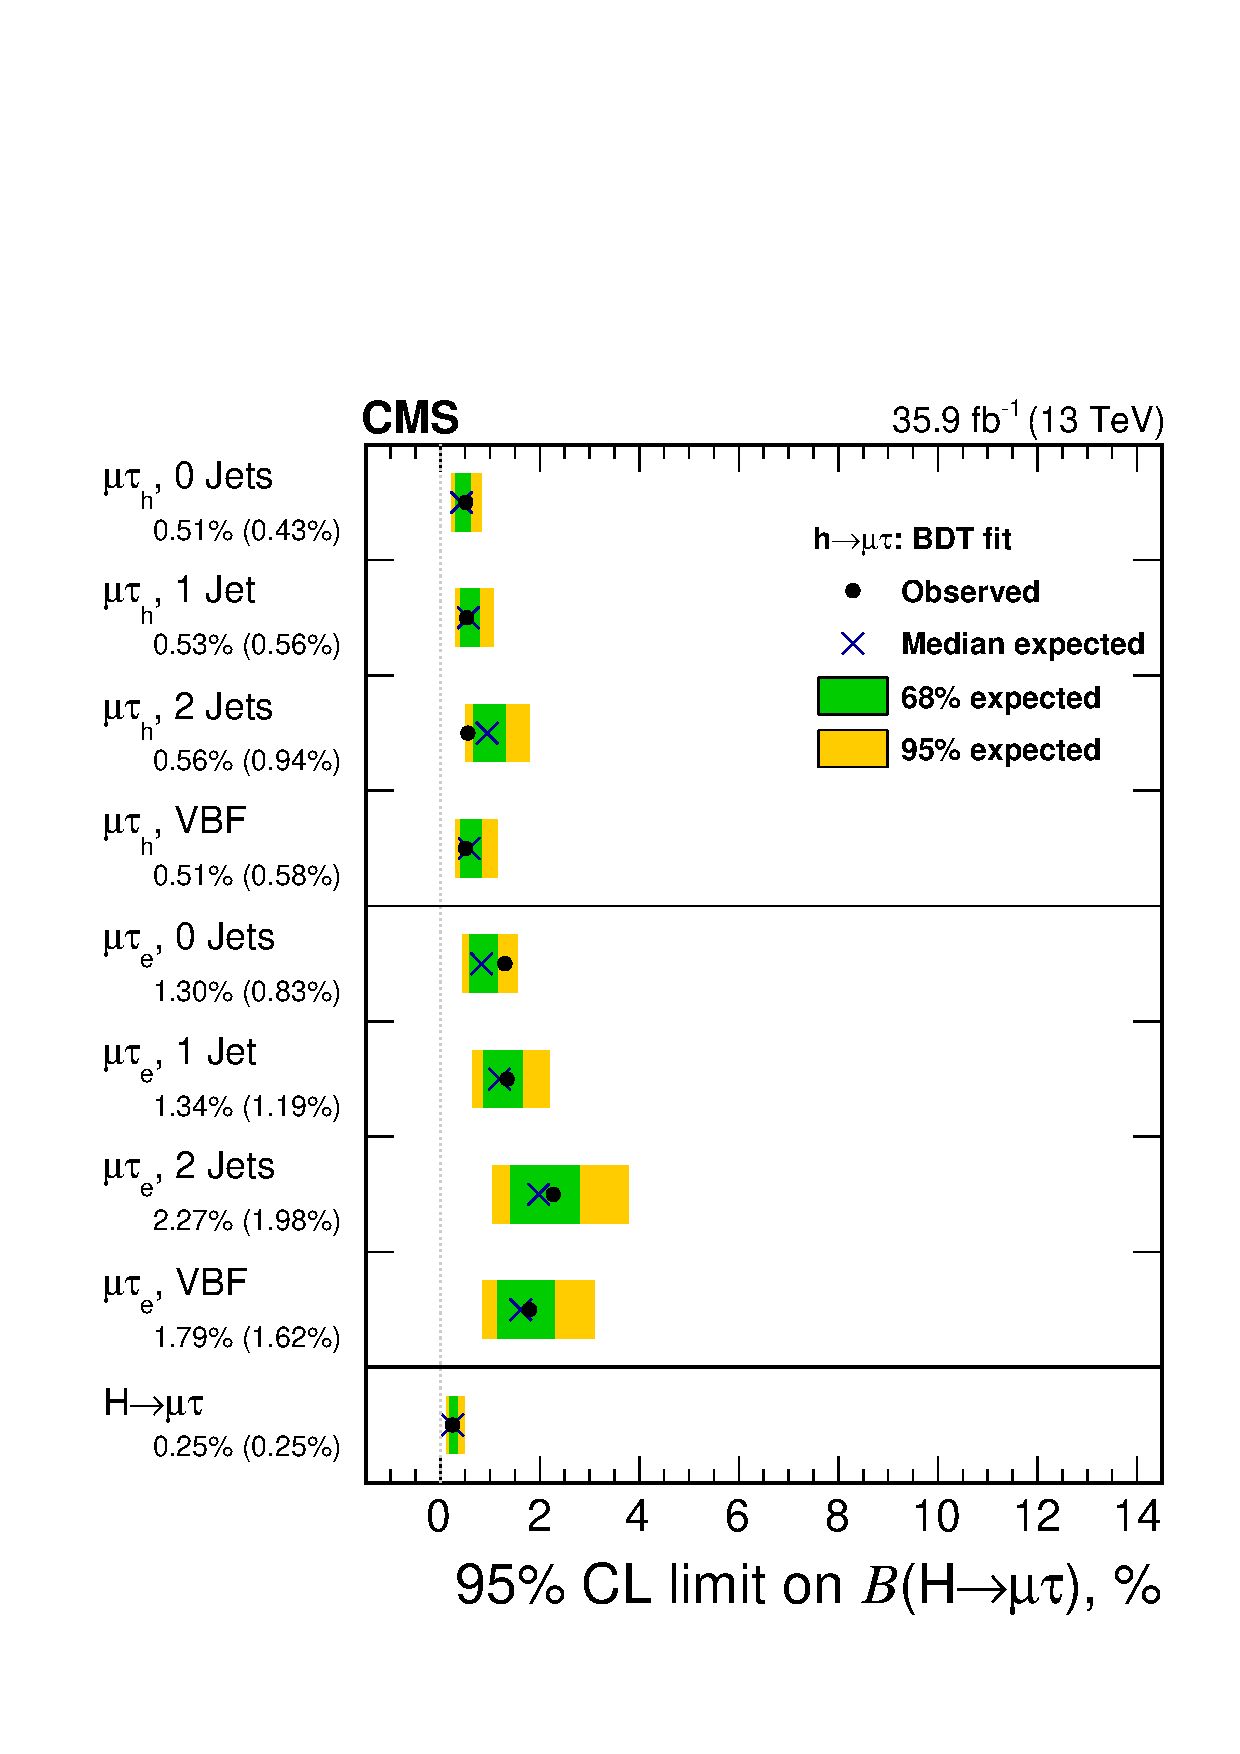
\includegraphics[width=0.45\textwidth]{plots/chapter2/BHmt.pdf}
  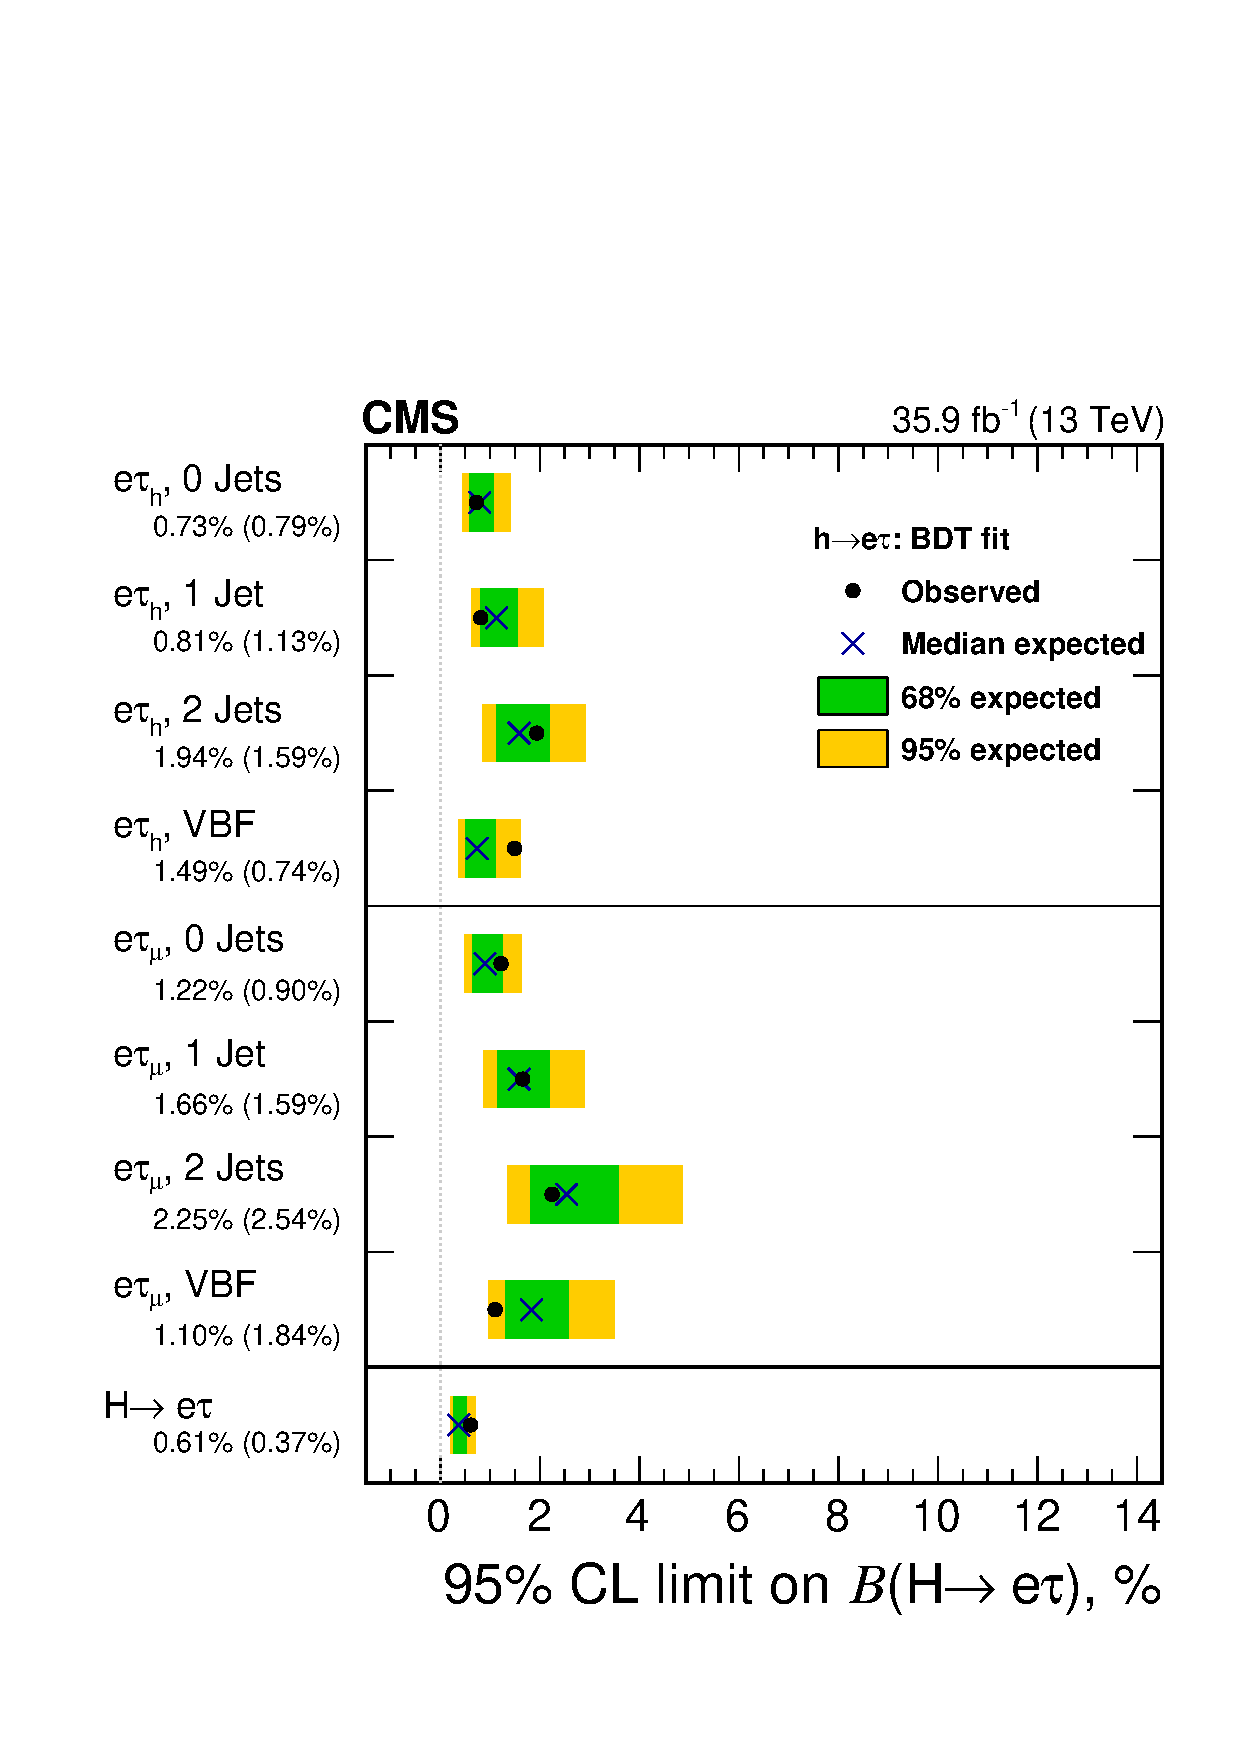
\includegraphics[width=0.45\textwidth]{plots/chapter2/BHet.pdf}
  \caption{Expected and observed 95\% CL upper limits for each category and their combination of the search performed by the CMS experiment~\cite{Sirunyan:2019shc}.}
  \label{fig:bh}
\end{figure}

\begin{figure}[htbp]
  \centering
  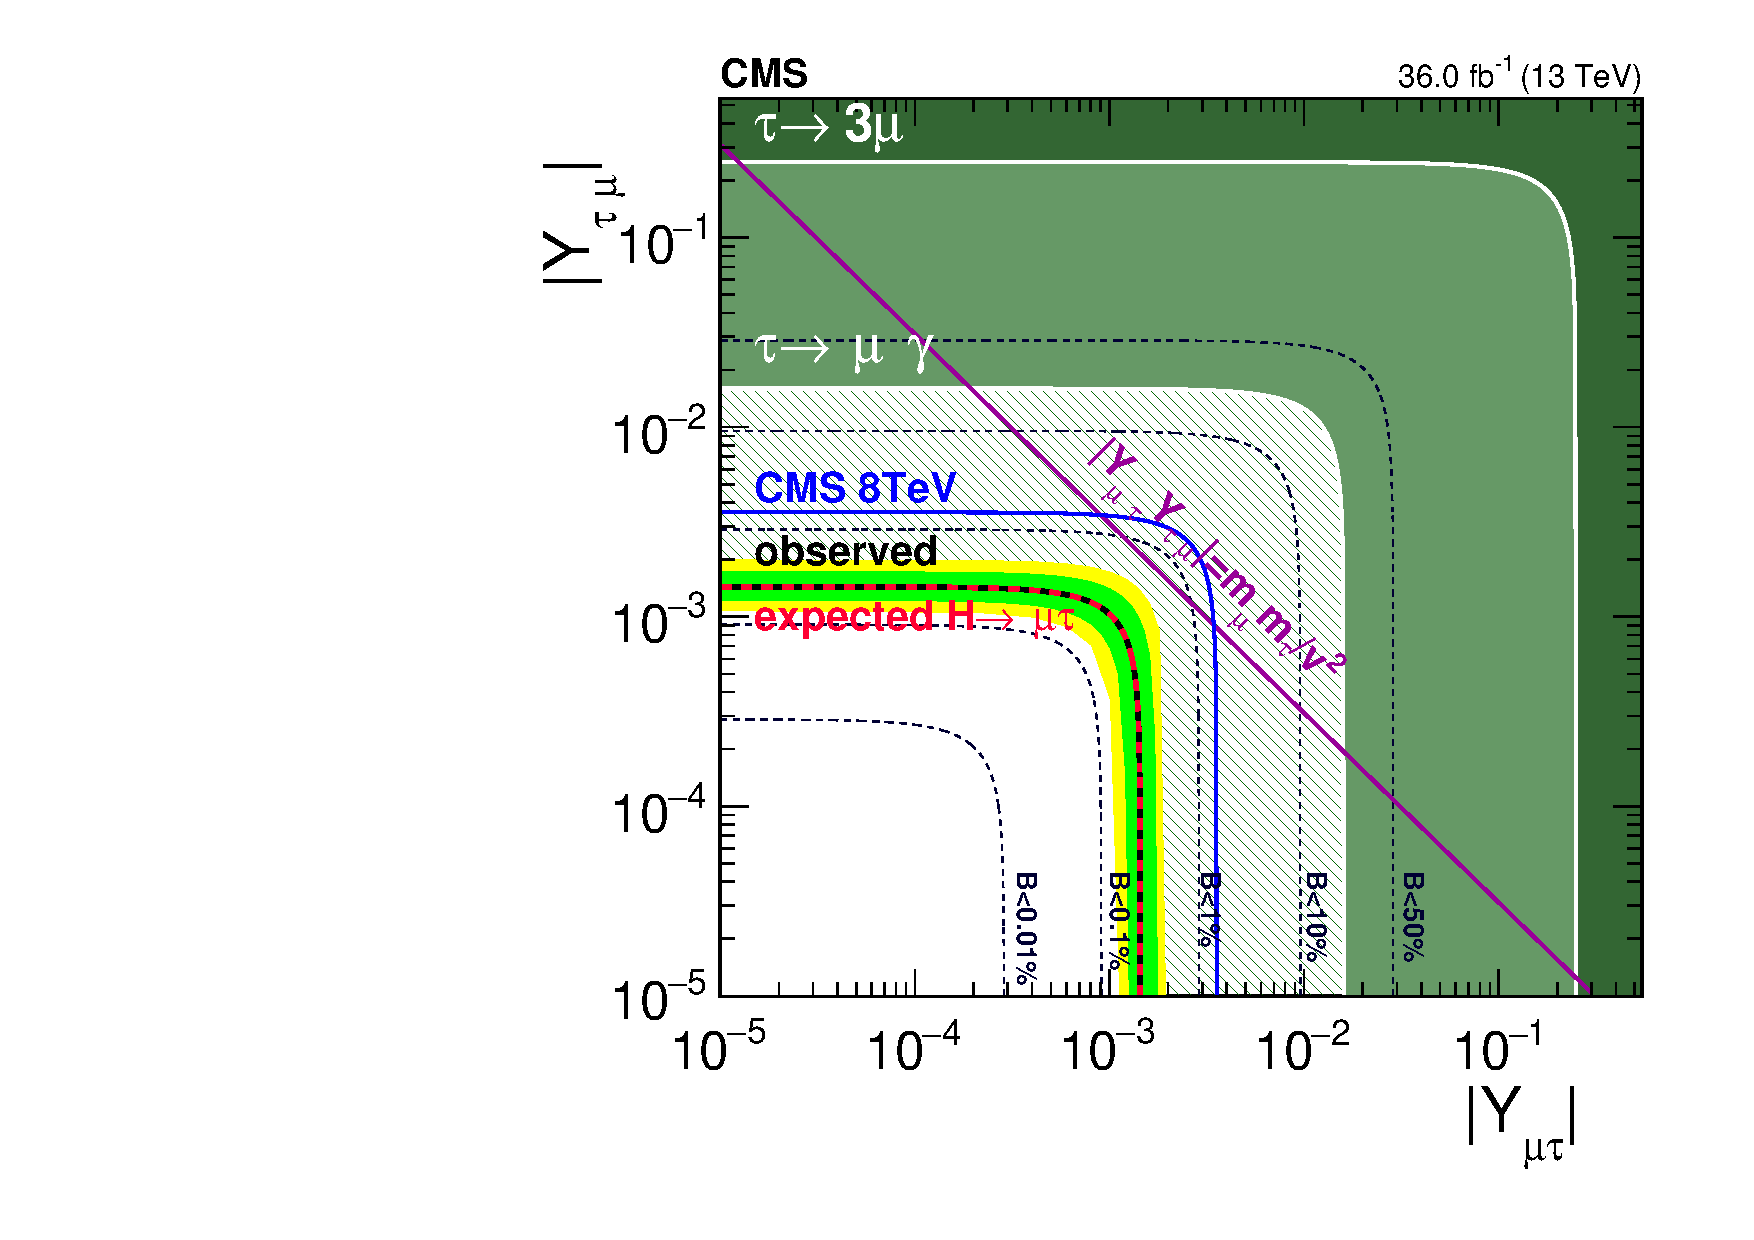
\includegraphics[width=0.45\textwidth]{plots/chapter2/Ymt.pdf}
  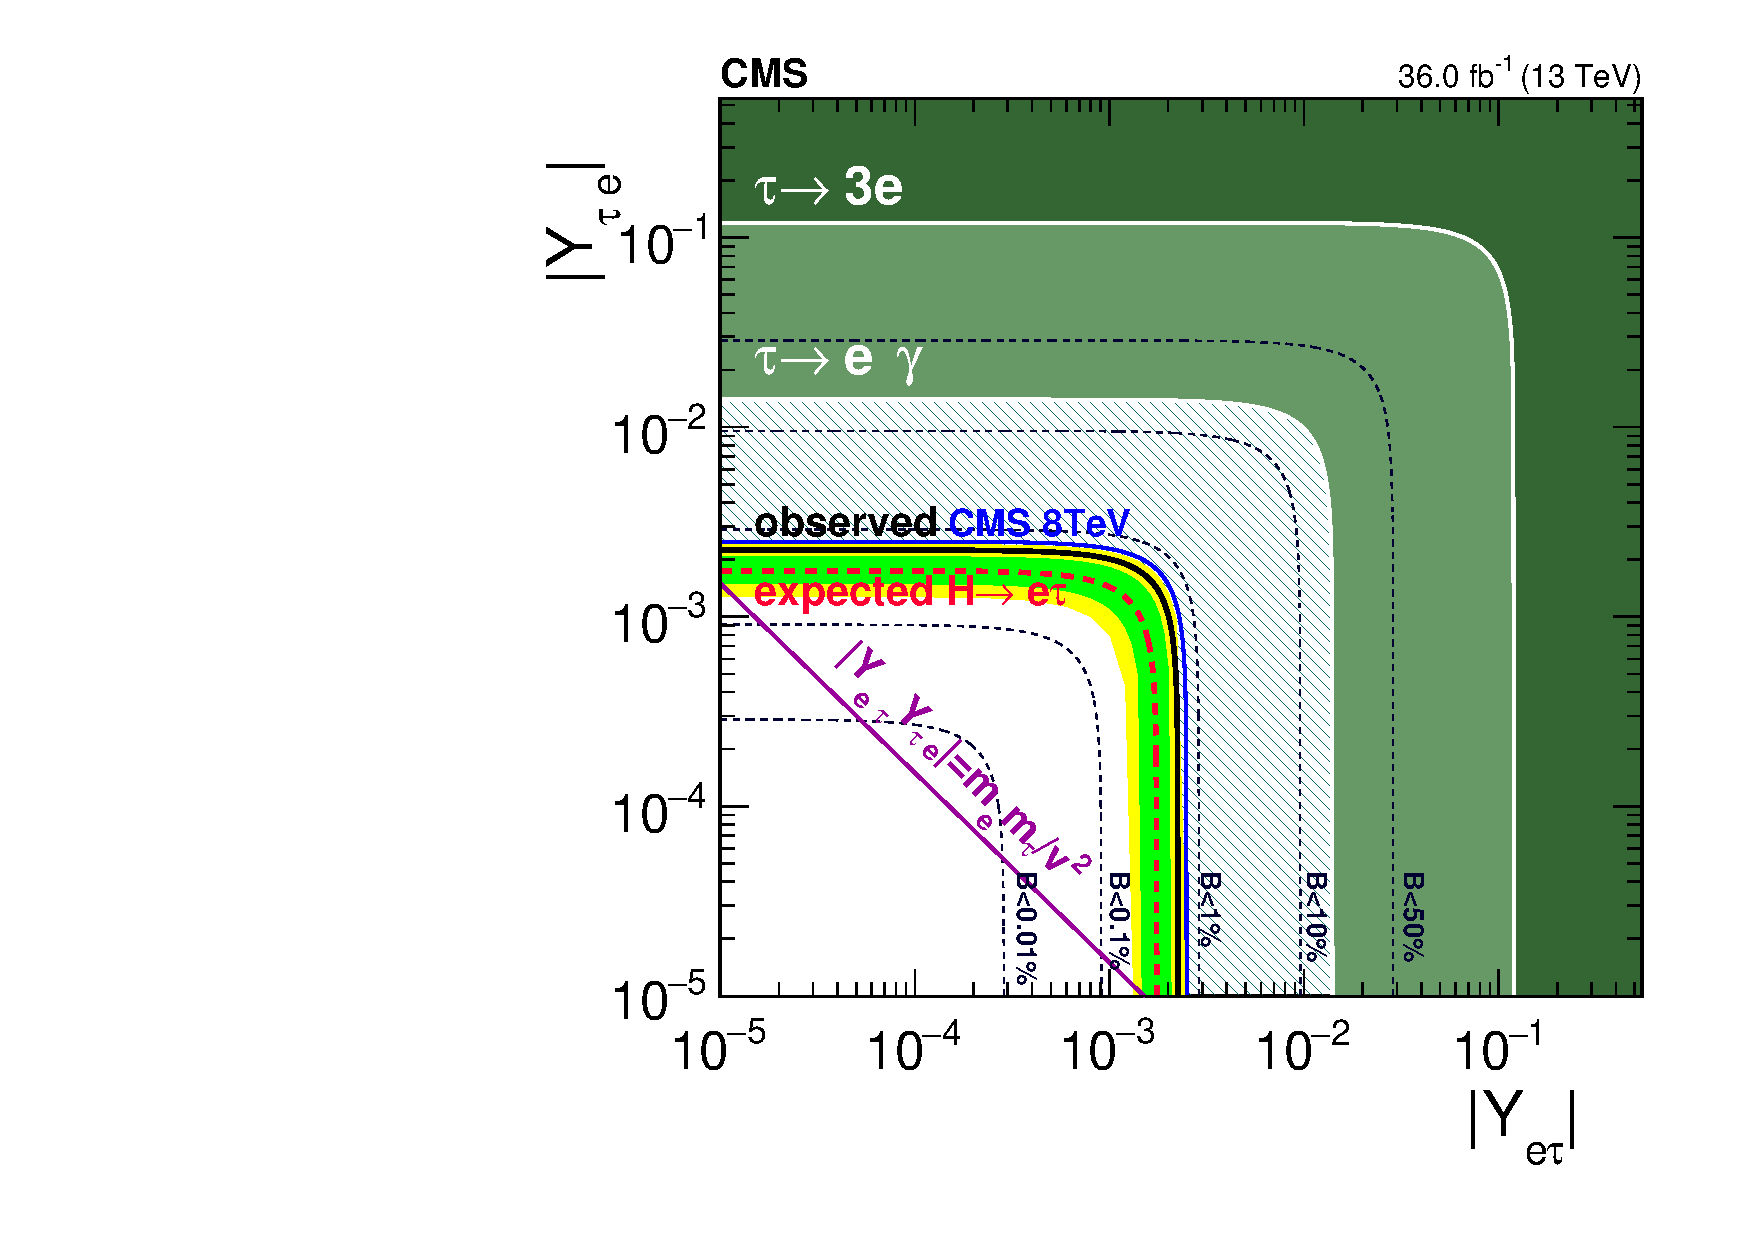
\includegraphics[width=0.45\textwidth]{plots/chapter2/Yet.pdf}
  \caption{Constraints on the LFV Yukawa couplings, $\Ymutau-\Ytaumu$ (left), and $\Yetau-\Ytaue$ (right) of the search performed by the CMS experiment.}
  \label{fig:yukawa}
\end{figure}
